
\chapter{Introduction}

\textrm{\glspl{infosystem}} are omnipresent in today's world, and being connected to the Web is more a common attribute than a special quality among them.
As a consequence, the Web is an ever growing institution in all aspects that it covers.
The number of data and functionality providing \textrm{\glspl{infosystem}} is growing in the whole spectrum from bigger computing centers down to smaller devices.
Computing centers are growing in size and quantity and they allow for massive amounts of data to be stored and accessed, moreover they also enable the construction and offering of more complex functionality.
At the same time, an increasing number of ever smaller devices also provides more \textrm{\glspl{infosystem}} attached to the Web.
Many of them are offering access to the Web itself, granting even more devices access and thus leverage the effect of the growing Web, e.g. mobile phones can act as a hotspot to grant Web access to other devices over \textrm{WiFi}.
A recent observed trend is all the smart things, which have access to the Web and start to form the \textrm{\gls{webofthings}}.
Today, these smart things can be everything from a temperature sensor to all the electronic devices within a house.
They do not only provide sensor data but they can also be controlled over the Web.
All these different types of services available on the Web make it a heterogeneous collection of \textrm{\glspl{infosystem}} and their services.
Great efforts are made to turn them into uniformly accessible \textrm{\glspl{webresource}}, e.g. the \textrm{\gls{semanticweb}} is a widely supported initiative towards a machine-readable, structured and semantically descripted Web.

Confronted with this rapid growth of the Web, an increasing number of human beings is exposed to it in their daily life, and they get literally flooded with informations and means to retrieve or process them.
Even though users have access to so many \textrm{\glspl{webresource}}, they often lack the knowledge, necessary time or right approach to weave them together.
Great value would be added for them if they could automatically get appropriate informations, in the right moment and in a condensed matter that supports them best.
They should be able to automate tedious tasks, e.g. detecting relevant changes in their preferred \textrm{\glspl{webresource}} and react on behalf of such changes.
This requires the identification of and filtering for user-relevant changes, appropriate timing, assembly and finally the placement of the outcome in the user's preferred \textrm{\glspl{webresource}}.

With the many existing \textrm{\glspl{infosystem}} and their services on the Web, users don't want to be bound to specific ones for certain tasks, as it is often the case nowadays.
They want to use the functionality or data of their preferred ones, which helps them best to fulfill their needs.
Hence, users should have to be able to create their own specific but still flexible \textrm{\gls{webresource}} orchestrations.
Since the need of users to orchestrate different services has gotten a lot of attention, some of the \textrm{\glspl{infosystem}} on the Web offer ways to spread their data to others, but in a limited way.
For example it is common for social network applications to push user-specific notifications to other social networks, e.g. singing in at a place in \textrm{Foursquare} can also be posted directly to the \textrm{Facebook} timeline.
Because of existing limitations, such as customizability or action imposing on \textrm{\gls{infosystem}} of their choice, users still end up mixing data and functionality from different \textrm{\glspl{webresource}} by hand, which often means to execute similar tasks repeatedly by hand.
Moreover the manual reaction on changes is deferred because the changes are not detected in real-time by the user or because the user is not able to react in a timely fashion.

Since data and functionality already exist in the Web, the users are theoretically enabled to automate their work to some extent by orchestrating those \textrm{\glspl{webresource}}.
Even though the access to resources gets simpler, the average user is still not capable to fully exploit the Web's full potential.
Another challenge is, that often a lot of effort has to be made, in understanding how the specific service works, before it can be fully exploited.
There is a lot of research that goes towards an easy to orchestrate the Web, but they are either often complicated to wield themselves, mere data copy tasks or static \textrm{\gls{webresource}} compositions.
Our goal is to enable user-defined resource orchestrations, and still exploiting their full potential by not limiting the set of their functionality and thus going towards a reactive Web.

A big part of the data, that becomes available to the users, is short-lived data that corresponds to state changes, which are changes in the \textrm{\glspl{infospace}} and can be modeled as events for detection or actions for imposition.
In this thesis we introduce an event-driven conceptual model that uses the programmability of \textrm{\glspl{infosystem}} and their services in order to impose reactivity between them.
By regarding the whole Web as an \textrm{\gls{infospace}}, in which we listen for triggered events and on which we impose actions as a result of user-defined rules, we are able to model a real-time reactive Web.
Such a personalized reactivity allows the orchestration of the Web and a tool to govern its data flood by automating tedious tasks.
Current \textrm{\gls{webresource}} orchestrations concentrate on data flow rather than on event flow, which are mere copy/paste tasks of data than smart reactivity.
This makes us believe that our event-based conceptual model can overcome certain shortcomings of the existing approaches and provides a step towards the real-time reactive Web.


\begin{figure}[!ht]
  \centering
  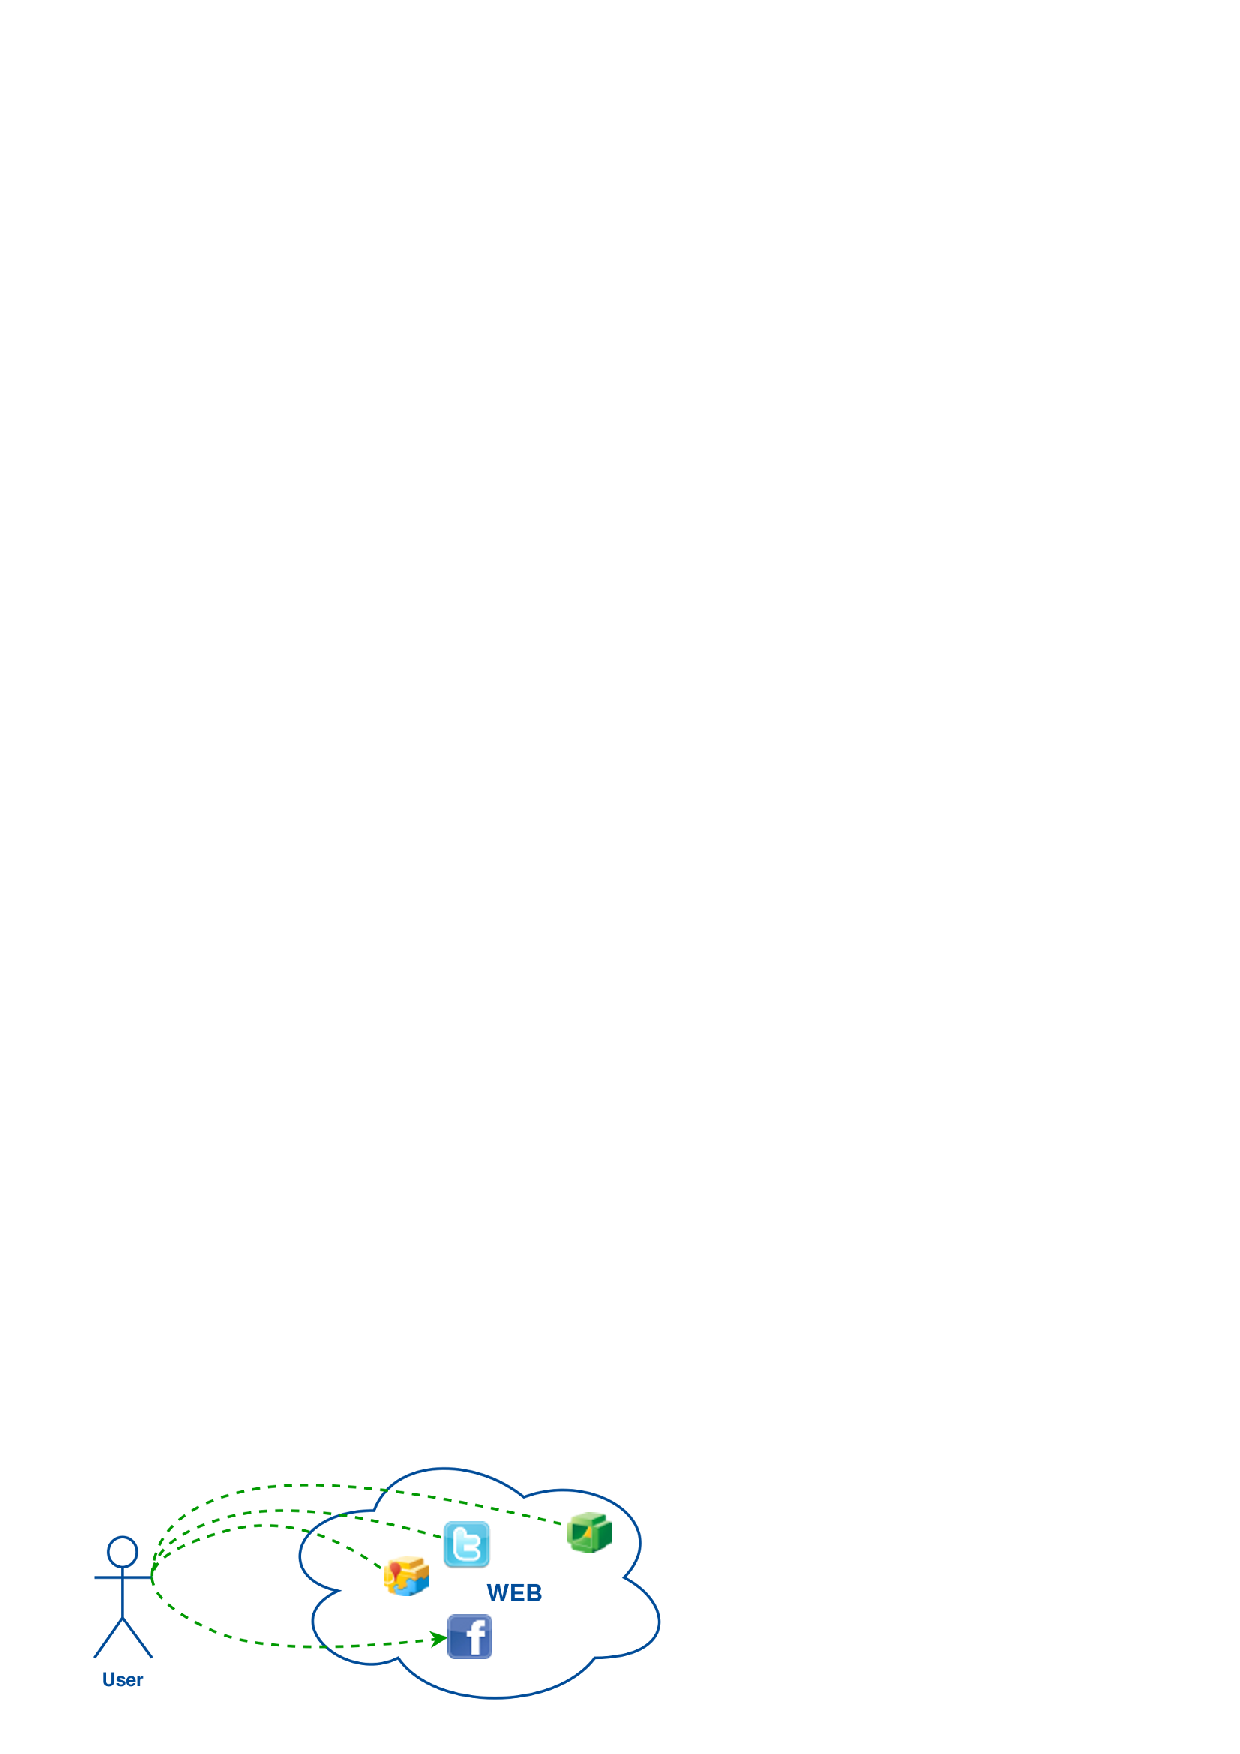
\includegraphics[width=0.7\textwidth]{figures/UsersWeildServicesInTheWeb}
  \caption{Users orchestrate the Web's Data and Functionality (... TODO prettify!)}
  \label{fig:UsersWeildServicesInTheWeb}
\end{figure}
% \textit{\small{MAKE NEW ONE! Figure with user orchestrating Web Resources}}
% \textit{\small{ewwww ugly figure....\\
% TODO show more concrete example with aha effect, light bulb. maybe parallel or serial events that turn into a result}}


% \textit{\small{TODO: use the word task or workflow?}}

